%%%%%%%%%%%%%%%%%%%%%%%%%%%%%%%%%%%%%%%%%%%%%%%%%%%%%%%%%%%%%%%%%%%%%%
% Problem statement
\begin{statement}[
  problempoints=70,
  timelimit=1 sekunda,
  memorylimit=512 MiB,
]{Slagalica}

Mali Fabijan je za rođendan dobio jednodimenzionalnu slagalicu koja se sastoji
od $N$ komadića. Primijetio je da svaki komadić ima jedan od sljedećih oblika:
\\

\begin{figure}[H]
\centering
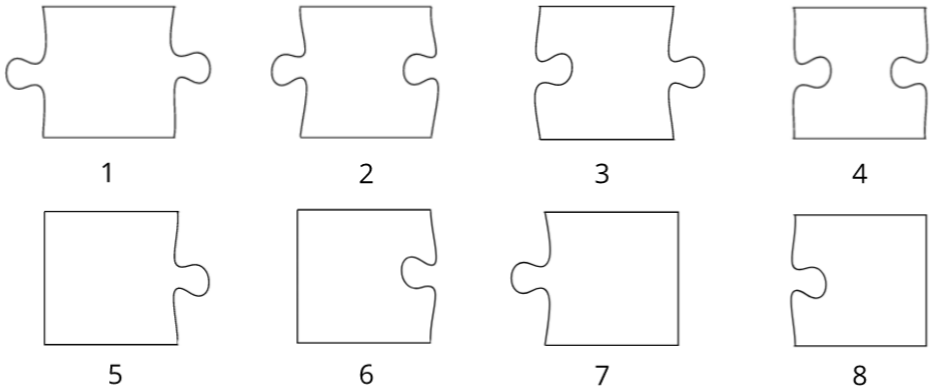
\includegraphics[width=0.6\textwidth]{img/puzzledef.png}
\end{figure}

Dodatno, poznato je da se među tih $N$ komadića nalazi točno jedan jedan komadić
oblika $5$ ili $6$ te točno jedan komadić oblika $7$ ili $8$.

Fabijan želi složiti sve komadiće u jednodimenzionalni slijed tako da prvi
komadić u slijedu bude oblika $5$ ili $6$, a zadnji oblika $7$ ili $8$.
Dva komadića može spojiti samo ako na rubu na kojem se dodiruju imaju suprotne
oblike, dakle jedan ima udubinu, a drugi izbočinu.

Budući da mu je to prelagano, Fabijan je na svaki komadić napisao različit
prirodan broj te se nakon toga zapitao kako bi trebao posložiti komadiće ako
želi da niz što ga redom čine brojevi zapisani na komadićima nakon slaganja bude
što manji. Niz $A$ je manji od niza $B$ ako za prvu poziciju $i$ na kojoj se
njihovi elementi razlikuju vrijedi $A_i$ < $B_i$.

\textbf{Napomena:} Komadići se ne smiju rotirati.

%%%%%%%%%%%%%%%%%%%%%%%%%%%%%%%%%%%%%%%%%%%%%%%%%%%%%%%%%%%%%%%%%%%%%%
% Input
\subsection*{Ulazni podaci}
U prvom je retku prirodan broj $N$ $(2 \le N \le 10^5)$ iz teksta zadatka.

U sljedećih su $N$ redaka dva prirodna broja $X_i$ $(1 \le X_i \le 8)$ i $A_i$
$(1 \le A_i \le 10^9)$, oblik $i$-tog komadića i broj koji je Fabijan napisao na
njega. Brojevi $A_i$ će biti međusobno različiti.

%%%%%%%%%%%%%%%%%%%%%%%%%%%%%%%%%%%%%%%%%%%%%%%%%%%%%%%%%%%%%%%%%%%%%%
% Output
\subsection*{Izlazni podaci}
Ako Fabijan može složiti slagalicu, potrebno je ispisati redom brojeve na
komadićima u složenoj slagalici koji tvore najmanji niz.

Ako Fabijan ne može složiti slagalicu, potrebno je ispisati $-1$.

%%%%%%%%%%%%%%%%%%%%%%%%%%%%%%%%%%%%%%%%%%%%%%%%%%%%%%%%%%%%%%%%%%%%%%
% Scoring
\subsection*{Bodovanje}
U test podacima ukupno vrijednima $5$ bodova vrijedi $N \le 4$.\\
U test podacima vrijednima dodatnih $5$ bodova vrijedi $N \le 10$.\\
U test podacima vrijednima dodatnih $10$ bodova neće se pojaviti komadići oblika $2$ i $3$.\\
U test podacima vrijednima dodatnih $20$ bodova bit će najviše jedan komadić oblika $1$ ili $4$.

Ako za neki testni primjer Fabijan može složiti slagalicu i vi ispišete ispravno
slaganje, ali niz nije najmanji, ostvarit ćete $40\%$ predviđenih bodova za taj
testni primjer.


%%%%%%%%%%%%%%%%%%%%%%%%%%%%%%%%%%%%%%%%%%%%%%%%%%%%%%%%%%%%%%%%%%%%%%
\subsection*{Probni primjeri}
\begin{tabularx}{\textwidth}{X'X'X}
\sampleinputs{test/slagalica.dummy.in.1}{test/slagalica.dummy.out.1} &
\sampleinputs{test/slagalica.dummy.in.2}{test/slagalica.dummy.out.2} &
\sampleinputs{test/slagalica.dummy.in.3}{test/slagalica.dummy.out.3}
\end{tabularx}

\textbf{Pojašnjenje prvog probnog primjera:}\\
Fabijan komadiće slagalice može složiti na dva različita načina:\\

\begin{figure}[H]
\centering
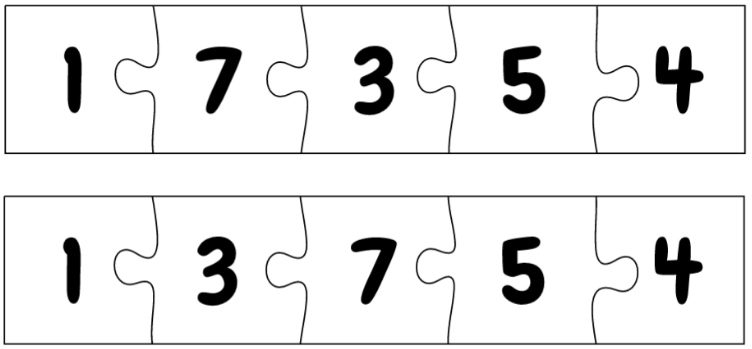
\includegraphics[width=0.6\textwidth]{img/sample_clarification.png}
\end{figure}
Vidimo da drugo slaganje na drugom komadiću slagalice ima manji broj pa je to
rješenje.

%%%%%%%%%%%%%%%%%%%%%%%%%%%%%%%%%%%%%%%%%%%%%%%%%%%%%%%%%%%%%%%%%%%%%%
% We're done
\end{statement}

%%% Local Variables:
%%% mode: latex
%%% mode: flyspell
%%% ispell-local-dictionary: "croatian"
%%% TeX-master: "../hio.tex"
%%% End:
